
\documentclass[a4paper,12pt]{article}
\usepackage[utf8]{inputenc}
\usepackage[a4paper,
            bindingoffset=0.2in,
            left=1in,
            right=1in,
            top=1in,
            bottom=1in,
            footskip=.25in]{geometry}


%###############################################################################

%\input{~/layout/global_layout}


%###############################################################################

% packages begin

\usepackage[
  backend=biber,
  sortcites=true,
  style=alphabetic,
  eprint=true,
  backref=true
]{biblatex}
\addbibresource{bibliography.bib}

\usepackage{euscript}[mathcal]
% e.g. \mathcal{A} for fancy letters in mathmode
\usepackage{amsmath,amssymb,amstext,amsthm}

\usepackage{mdframed}
\newmdtheoremenv[nobreak=true]{problem}{Problem}[subsection]
\newmdtheoremenv[nobreak=true]{claim}{Claim}[subsection]
\newtheorem{definition}{Definition}[subsection]
\newtheorem{lemma}{Lemma}[claim]
\newtheorem{plemma}{Lemma}[problem]

\usepackage{mathtools}
\DeclarePairedDelimiter\ceil{\lceil}{\rceil}
\DeclarePairedDelimiter\floor{\lfloor}{\rfloor}

\usepackage{enumerate}
\usepackage[pdftex]{graphicx}
\usepackage{subcaption}
% 'draft' für schnelleres rendern mitübergeben -> [pdftex, draft]
% dadruch wird nicht das bild mitgerendered, sondern nur ein kasten mit bildname -> schont ressourcen

\usepackage{hyperref}

\usepackage{tikz}
\usetikzlibrary{arrows,automata,matrix,positioning,shapes}

% for adding non-formatted text to include source-code
\usepackage{listings}
\lstset{language=Python,basicstyle=\footnotesize}
% z.B.:
% \lstinputlisting{source_filename.py}
% \lstinputlisting[lanugage=Python, firstline=37, lastline=45]{source_filename.py}
%
% oder
%
% \begin{lstlisting}[frame=single]
% CODE HERE
%\end{lstlisting}
\usepackage{algorithm}
\usepackage{algpseudocode}

\usepackage{wasysym}

\usepackage{titling}
\usepackage{titlesec}
\usepackage[nocheck]{fancyhdr}
\usepackage{lastpage}

\usepackage{kantlipsum}
\usepackage[colorinlistoftodos,prependcaption,textsize=tiny]{todonotes}

% packages end
%###############################################################################

\pretitle{% add some rules
  \begin{center}
    \LARGE\bfseries
} %, make the fonts bigger, make the title (only) bold
\posttitle{%
  \end{center}%
  %\vskip .75em plus .25em minus .25em% increase the vertical spacing a bit, make this particular glue stretchier
}
\predate{%
  \begin{center}
    \normalsize
}
\postdate{%
  \end{center}%
}

\titleformat*{\section}{\Large\bfseries}
\titleformat*{\subsection}{\large\bfseries}
\titleformat*{\subsubsection}{\normalsize\bfseries}

\titleformat*{\paragraph}{\Large\bfseries}
\titleformat*{\subparagraph}{\large\bfseries}

%###############################################################################
% TODO define Headers and Fotter

\pagestyle{fancy}
\fancyhf{}
% l=left, c=center, r=right; e=even_pagenumber, o=odd_pagenumber; h=header, f=footer
% example: [lh] -> left header, [lof,ref] -> fotter left when odd, right when even
%\fancyhf[lh]{}
%\fancyhf[ch]{}
%\fancyhf[rh]{}
%\fancyhf[lf]{}
\fancyhf[cf]{\footnotesize Page \thepage\ of \pageref*{LastPage}}
%\fancyhf[rf]{}
\renewcommand{\headrule}{} % removes horizontal header line

% Fotter options for first page

\fancypagestyle{firstpagestyle}{
  \renewcommand{\thedate}{\textmd{}} % removes horizontal header line
  \fancyhf{}
  \fancyhf[lh]{\ttfamily M.Sc. Computer Science\\KTH Royal Institute of Technology}
  \fancyhf[rh]{\ttfamily Period 2\\\today}
  \fancyfoot[C]{\footnotesize Page \thepage\ of \pageref*{LastPage}}
  \renewcommand{\headrule}{} % removes horizontal header line
}
%###############################################################################
% Todo: define Title

\title{
  \normalsize{DD2358 VT25 Introduction to}\\
  \normalsize{High Performance Computing}\\
  \large{Assignment X}\\
}
\author{
  \small Author 1\\[-0.75ex]
%  \footnotesize\texttt{MN: }\\[-1ex]
  \scriptsize\texttt{xx@kth.se}
  \and
  \small Author 2\\[-0.75ex]
%  \footnotesize\texttt{MN: }\\[-1ex]
  \scriptsize\texttt{xx@kth.se}
  \and
  \small Author 3\\[-0.75ex]
%  \footnotesize\texttt{MN: }\\[-1ex]
  \scriptsize\texttt{xx@kth.se}
  \and
  \small Paul Mayer\\[-0.75ex]
%  \footnotesize\texttt{MN: }\\[-1ex]
  \scriptsize\texttt{pmayer@kth.se}
}
\date{}

%###############################################################################
% define Commands

\newcommand{\N}{\mathbb{N}}
\newcommand{\R}{\mathbb{R}}
\newcommand{\Z}{\mathbb{Z}}
\newcommand{\I}{\mathbb{I}}

\newcommand{\E}{\mathbb{E}}
\newcommand{\Prob}{\mathbb{P}}

\renewcommand{\epsilon}{\varepsilon}

% Todo: Set Counter to Excercise Sheet Number
%\setcounter{section}{1}
%\setcounter{subsection}{1}

%###############################################################################
%###############################################################################

\begin{document}
\maketitle
\thispagestyle{firstpagestyle}

% \tableofcontents
\listoftodos

\vspace{1em}

%---
%
\section*{Prefix}
\todo[inline]{Make sure title and headers are correctly changed!}
\todo[inline]{Change Author names and mails.}

% content begin
%

\section{Profiling the Julia Set Code}
\subsection{Calculate the Clock Granularity of different Python Timers}
For profiling we used the method given on the exercise page.
On the Apple Silicon M1, I recieved the following output, using the best out of 1000 runs each:
%\texttt{\$ python ClockGranularity.py}\\
%\texttt{time.time: 7.152557373046875e-07 s}\\
%\texttt{time.time\_ns: 7.680000000000001e-07 s}\\
%\texttt{timeit.default\_timer: 8.300412446260452e-08 s}
\begin{lstlisting}[language=bash,basicstyle=\ttfamily]
  $ python ClockGranularity.py
  time.time: 7.152557373046875e-07 s
  time.time_ns: 7.680000000000001e-07 s
  timeit.default_timer: 8.300412446260452e-08 s
\end{lstlisting}

\subsection{Timing the Julia set code functions}
The M1-chip has a clock frequency of 3.2GHz.
\begin{lstlisting}[language=bash,basicstyle=\ttfamily]
  & python JuliaSet.py
  number of runs: 20
  desired width: 1000
  max iterations: 300

  calc_pure_python
      mean: 2.39370298139911 s
      std: 0.019263214648773588 s

  calculate_z_serial_purepython
      mean: 2.534685760299908 s
      std: 0.02066843684620983 s
\end{lstlisting}
The surprising observation to us is that the standard deviation is higher than we would expect.
With a clock frequency of 3.2GHz, a standard deviation of 0.02 s results in $32GHz \cdot 0.02s = 64\ 000\ 000$ clock cycles.
We suspect that this large difference in the number of clock cycles has to be the result of other processes taking up compute time.
This makes us believe that the difference is more the result of variations in system workload than the actual clock granularity.

\subsection{Profile the Julia set code with cProfile and line\_profiler the computation}

Here are the results for the cProfiler:
\begin{lstlisting}[language=bash,basicstyle=\scriptsize\ttfamily]
$ python -m cProfile -s cumulative JuliaSet.py
Length of x: 1000
Total elements: 1000000
width:	1000
output:	33219980
         36304066 function calls (36302053 primitive calls) in 5.498 seconds

   Ordered by: cumulative time

   ncalls  tottime  percall  cumtime  percall filename:lineno(function)
     93/1    0.000    0.000    5.498    5.498 {built-in method builtins.exec}
        1    0.013    0.013    5.498    5.498 JuliaSet.py:1(<module>)
        1    0.343    0.343    5.440    5.440 JuliaSet.py:25(calc_pure_python)
        1    3.468    3.468    4.951    4.951 JuliaSet.py:66(calculate_z_serial_purepython)
 34219980    1.483    0.000    1.483    0.000 {built-in method builtins.abs}
  2004574    0.142    0.000    0.142    0.000 {method 'append' of 'list' objects}
        8    0.000    0.000    0.118    0.015 __init__.py:1(<module>)
\end{lstlisting}

The \verb|line_profiler| returns:
\begin{lstlisting}[language=bash,basicstyle=\tiny\ttfamily]
$ python -m line_profiler JuliaSet.py.lprof
Timer unit: 1e-06 s

Total time: 23.4185 s
File: JuliaSet.py
Function: calc_pure_python at line 25

Line #      Hits         Time  Per Hit   % Time  Line Contents
==============================================================
    25                                           @profile
    26                                           def calc_pure_python(desired_width, max_iterations):
    27                                               Create a list of complex coordinates (zs) and complex parameters (cs),
    28                                               build Julia set
    29         1          1.0      1.0      0.0      x_step = (x2 - x1) / desired_width
    30         1          1.0      1.0      0.0      y_step = (y1 - y2) / desired_width
    31         1          0.0      0.0      0.0      x = []
    32         1          0.0      0.0      0.0      y = []
    33         1          0.0      0.0      0.0      ycoord = y2
    34      1001         94.0      0.1      0.0      while ycoord > y1:
    35      1000         81.0      0.1      0.0          y.append(ycoord)
    36      1000         92.0      0.1      0.0          ycoord += y_step
    37         1          0.0      0.0      0.0      xcoord = x1
    38      1001        115.0      0.1      0.0      while xcoord < x2:
    39      1000         82.0      0.1      0.0          x.append(xcoord)
    40      1000         87.0      0.1      0.0          xcoord += x_step
    41                                               # build a list of coordinates and the initial condition for each cell.
    42                                               # Note that our initial condition is a constant and could easily be removed,
    43                                               # we use it to simulate a real-world scenario with several inputs to our
    44                                               # function
    45         1          0.0      0.0      0.0      zs = []
    46         1          0.0      0.0      0.0      cs = []
    47      1001        130.0      0.1      0.0      for ycoord in y:
    48   1001000     111862.0      0.1      0.5          for xcoord in x:
    49   1000000     134319.0      0.1      0.6              zs.append(complex(xcoord, ycoord))
    50   1000000     137054.0      0.1      0.6              cs.append(complex(c_real, c_imag))
    51
    52         1         29.0     29.0      0.0      print("Length of x:", len(x))
    53         1          3.0      3.0      0.0      print("Total elements:", len(zs))
    54         1   23029180.0    2e+07     98.3      output = calculate_z_serial_purepython(max_iterations, zs, cs)
    55         1       2753.0   2753.0      0.0      print(f"width:\t{desired_width}\noutput:\t{sum(output)}")
    56
    57         1          1.0      1.0      0.0      if desired_width == 1000:
    58                                                   # This sum is expected for a 1000^2 grid with 300 iterations
    59         1       2633.0   2633.0      0.0          assert sum(output) == 33219980
    60                                               elif desired_width == 10000:
    61                                                   assert sum(output) == 3323787446
    62                                               else:
    63                                                   print("no asserts for this dimension...")

Total time: 12.0898 s
File: JuliaSet.py
Function: calculate_z_serial_purepython at line 66

Line #      Hits         Time  Per Hit   % Time  Line Contents
==============================================================
    66                                           @profile
    67                                           def calculate_z_serial_purepython(maxiter, zs, cs):
    68                                               """Calculate output list using Julia update rule"""
    69         1        875.0    875.0      0.0      output = [0] * len(zs)
    70   1000001     122094.0      0.1      1.0      for i in range(len(zs)):
    71   1000000      82909.0      0.1      0.7          n = 0
    72   1000000      98526.0      0.1      0.8          z = zs[i]
    73   1000000      78577.0      0.1      0.6          c = cs[i]
    74  34219980    5268274.0      0.2     43.6          while abs(z) < 2 and n < maxiter:
    75  33219980    3447190.0      0.1     28.5              z = z * z + c
    76  33219980    2903360.0      0.1     24.0              n += 1
    77   1000000      87992.0      0.1      0.7          output[i] = n
    78         1          1.0      1.0      0.0      return output
\end{lstlisting}

When analysing the two functions, we clearly see that most of the time spent is in the computation of the inner loop of the  \verb|calculate_z_serial_purepython| function (lines 74-76).
Over 40 \% of the time was spent computing the \verb|abs| function.

\begin{figure}[h!]
  \centering
  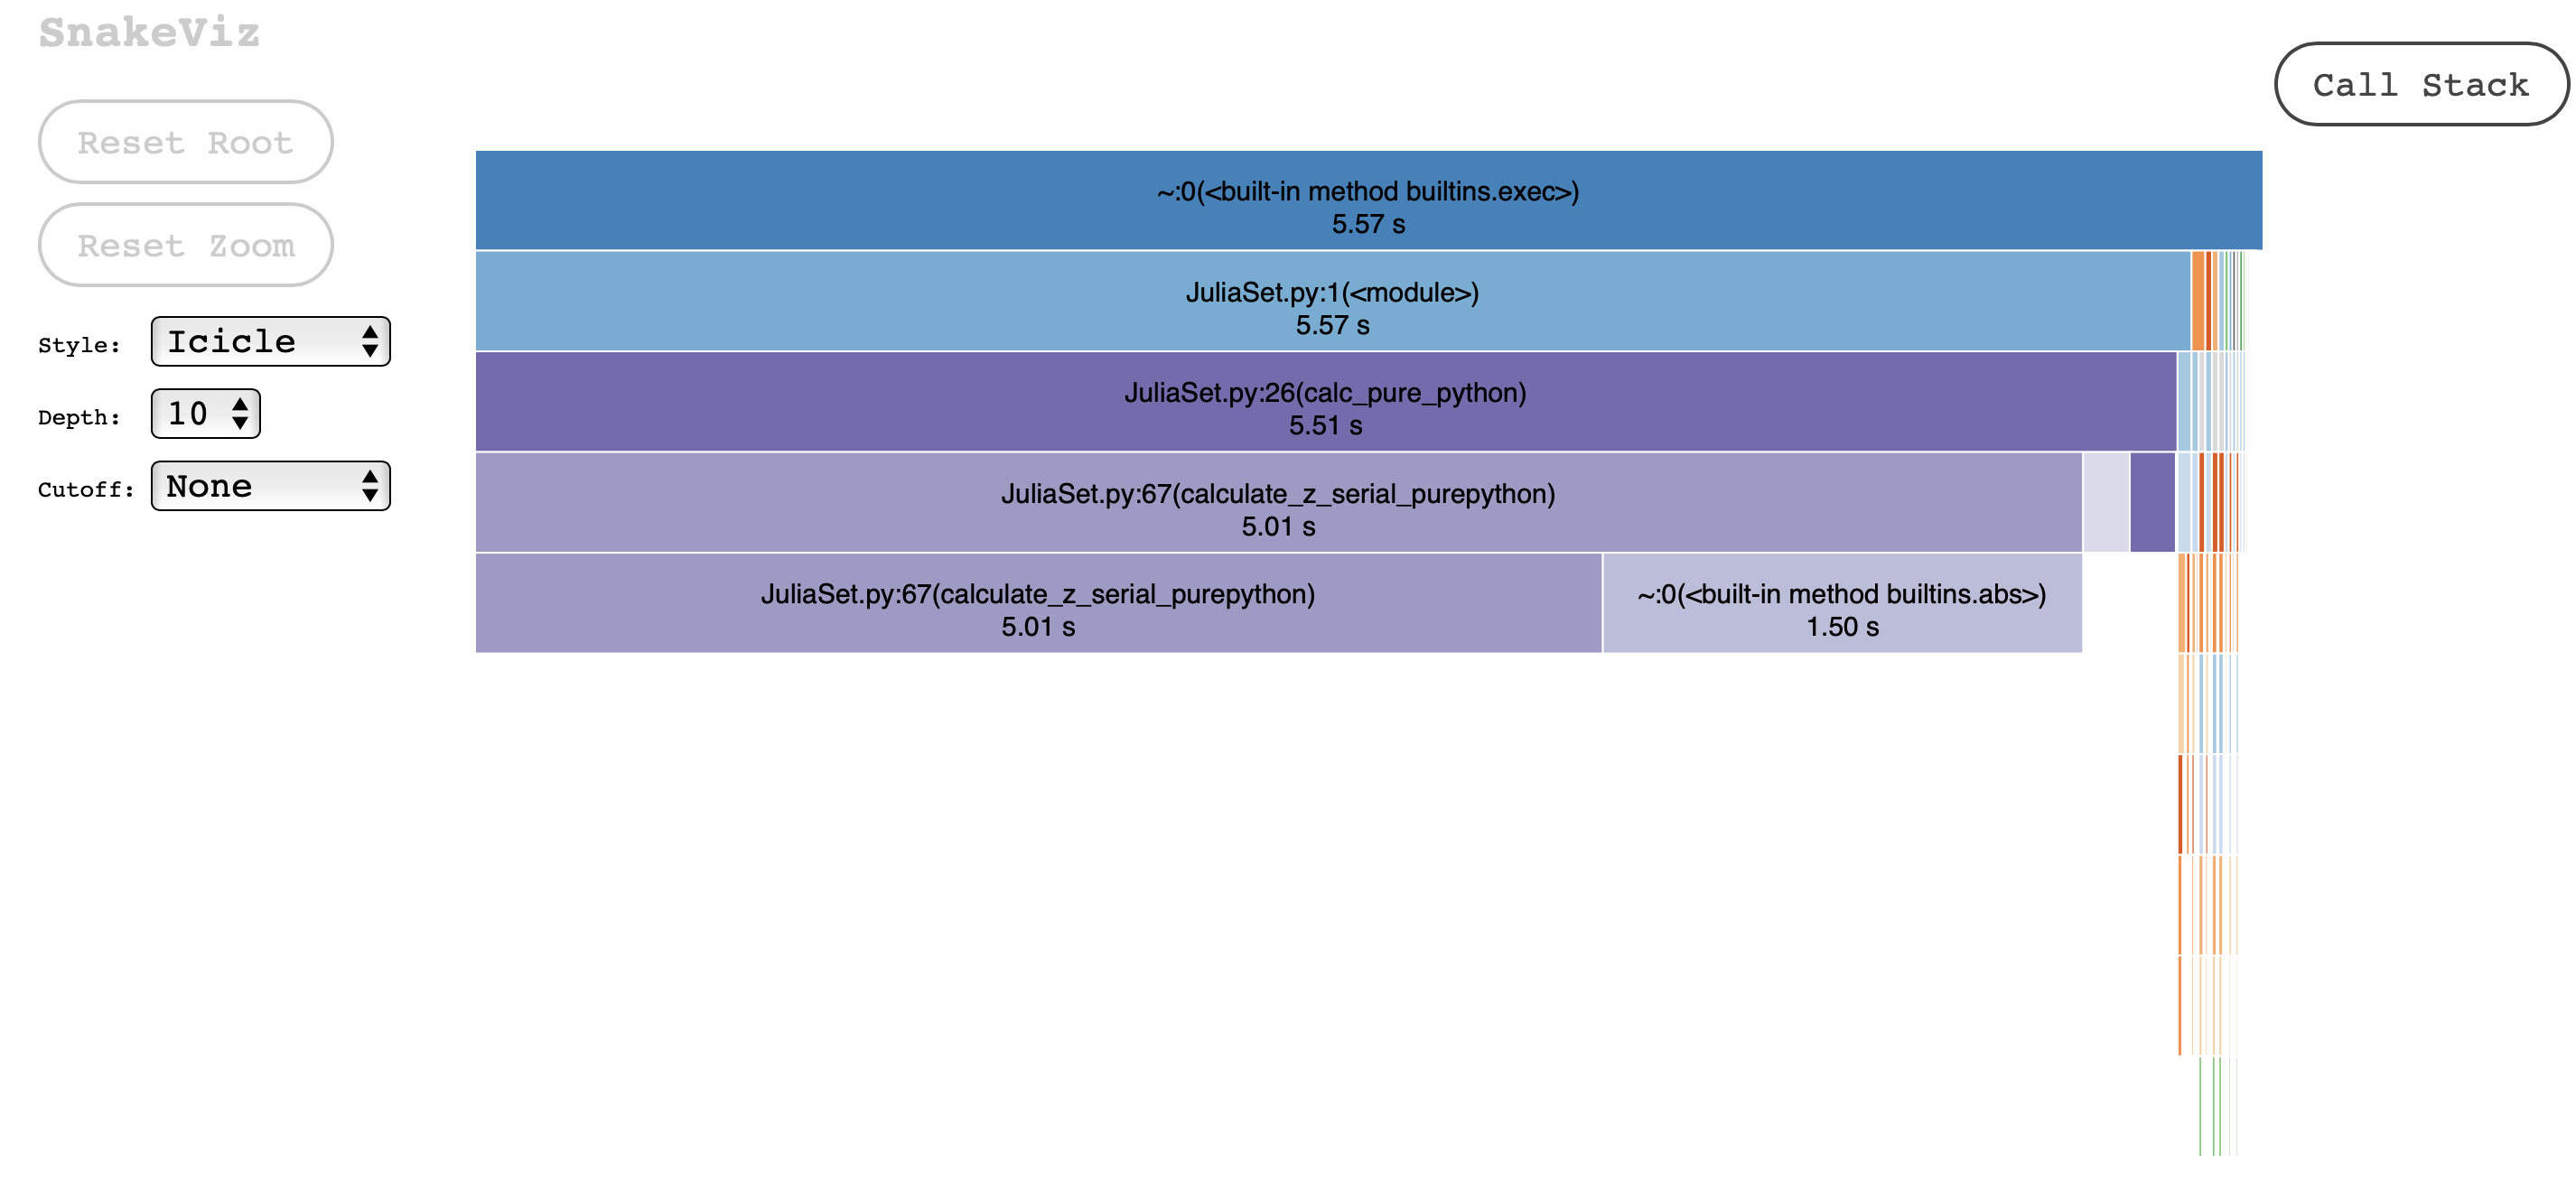
\includegraphics[width=\textwidth]{images/julia_snakeviz_view}
  \caption{Julia snakeviz view}
  \label{fig:julia-snakeviz}
\end{figure}

\textbf{Overhead:}
Running the \verb|JuliaSet| program without the profiler took $2.5 s$.
The overhead for using the \verb|cProfile| module were around 3 seconds slower.
That is over twice the runtime.

Results were even worse when using the \verb|line_profiler|.
The total runtime was around $23 s$, which is a magnitude higher than the original code.

\subsection{Memory-profile the Juliaset code. Use the memory\_profiler and mprof to profile the computation in JuliaSet code}

\verb|mprof| gives us the following result:
\begin{figure}[h!]
  \centering
  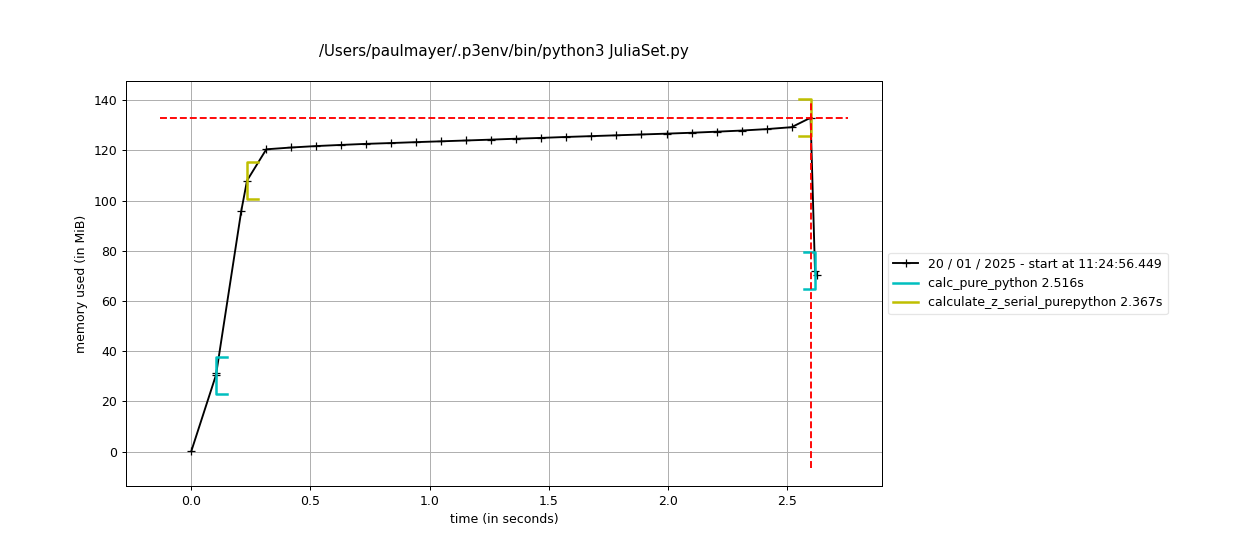
\includegraphics[width=\textwidth]{images/julia_mprofile}
  \caption{Julia mProfile}
  \label{fig:julia-mprofile}
\end{figure}

Using the line-by-line \verb|memory_profiler| returns:
\begin{lstlisting}[language=bash,basicstyle=\tiny\ttfamily]
Length of x: 100
Total elements: 10000
width:	100
output:	334236
no asserts for this dimension...
total calculation time: 15.793842832994414 s
Filename: JuliaSet.py

Line #    Mem usage    Increment  Occurrences   Line Contents
=============================================================
    25   29.625 MiB   29.625 MiB           1   @profile

    [...]

    47   30.328 MiB    0.000 MiB         101       for ycoord in y:
    48   30.328 MiB    0.016 MiB       10100           for xcoord in x:
    49   30.328 MiB    0.062 MiB       10000               zs.append(complex(xcoord, ycoord))
    50   30.328 MiB    0.625 MiB       10000               cs.append(complex(c_real, c_imag))
    51
    52   30.344 MiB    0.016 MiB           1       print("Length of x:", len(x))
    53   30.344 MiB    0.000 MiB           1       print("Total elements:", len(zs))
    54   30.531 MiB   30.531 MiB           1       output = calculate_z_serial_purepython(max_iterations, zs, cs)
    55   30.531 MiB    0.000 MiB           1       print(f"width:\t{desired_width}\noutput:\t{sum(output)}")

    [...]


Filename: JuliaSet.py

Line #    Mem usage    Increment  Occurrences   Line Contents
=============================================================
    66   30.344 MiB   30.344 MiB           1   @profile
    67                                         def calculate_z_serial_purepython(maxiter, zs, cs):
    68                                             """Calculate output list using Julia update rule"""
    69   30.453 MiB    0.109 MiB           1       output = [0] * len(zs)
    70   30.531 MiB    0.000 MiB       10001       for i in range(len(zs)):
    71   30.531 MiB    0.016 MiB       10000           n = 0
    72   30.531 MiB    0.000 MiB       10000           z = zs[i]
    73   30.531 MiB    0.000 MiB       10000           c = cs[i]
    74   30.531 MiB    0.016 MiB      344236           while abs(z) < 2 and n < maxiter:
    75   30.531 MiB    0.016 MiB      334236               z = z * z + c
    76   30.531 MiB    0.031 MiB      334236               n += 1
    77   30.531 MiB    0.000 MiB       10000           output[i] = n
    78   30.531 MiB    0.000 MiB           1       return output
\end{lstlisting}

\textbf{Overhead:}
Running \verb|mprof| did not show any significant overhead compared to unprofiled code.
However, running \verb|memory_profiler| increased the runtime by a shocking factor of $750$.

\newpage
\section{Profiling Diffusion Process Code}
\subsection{Profile the diffusion code with cProfile and line\_profiler the computation}

Using cProfile turned out to be not very insightful.
As expected, most of the time was spent in the \verb|evolve| method of the program; however, there was not much else insight we could draw from that.

\begin{figure}[h!]
  \centering
  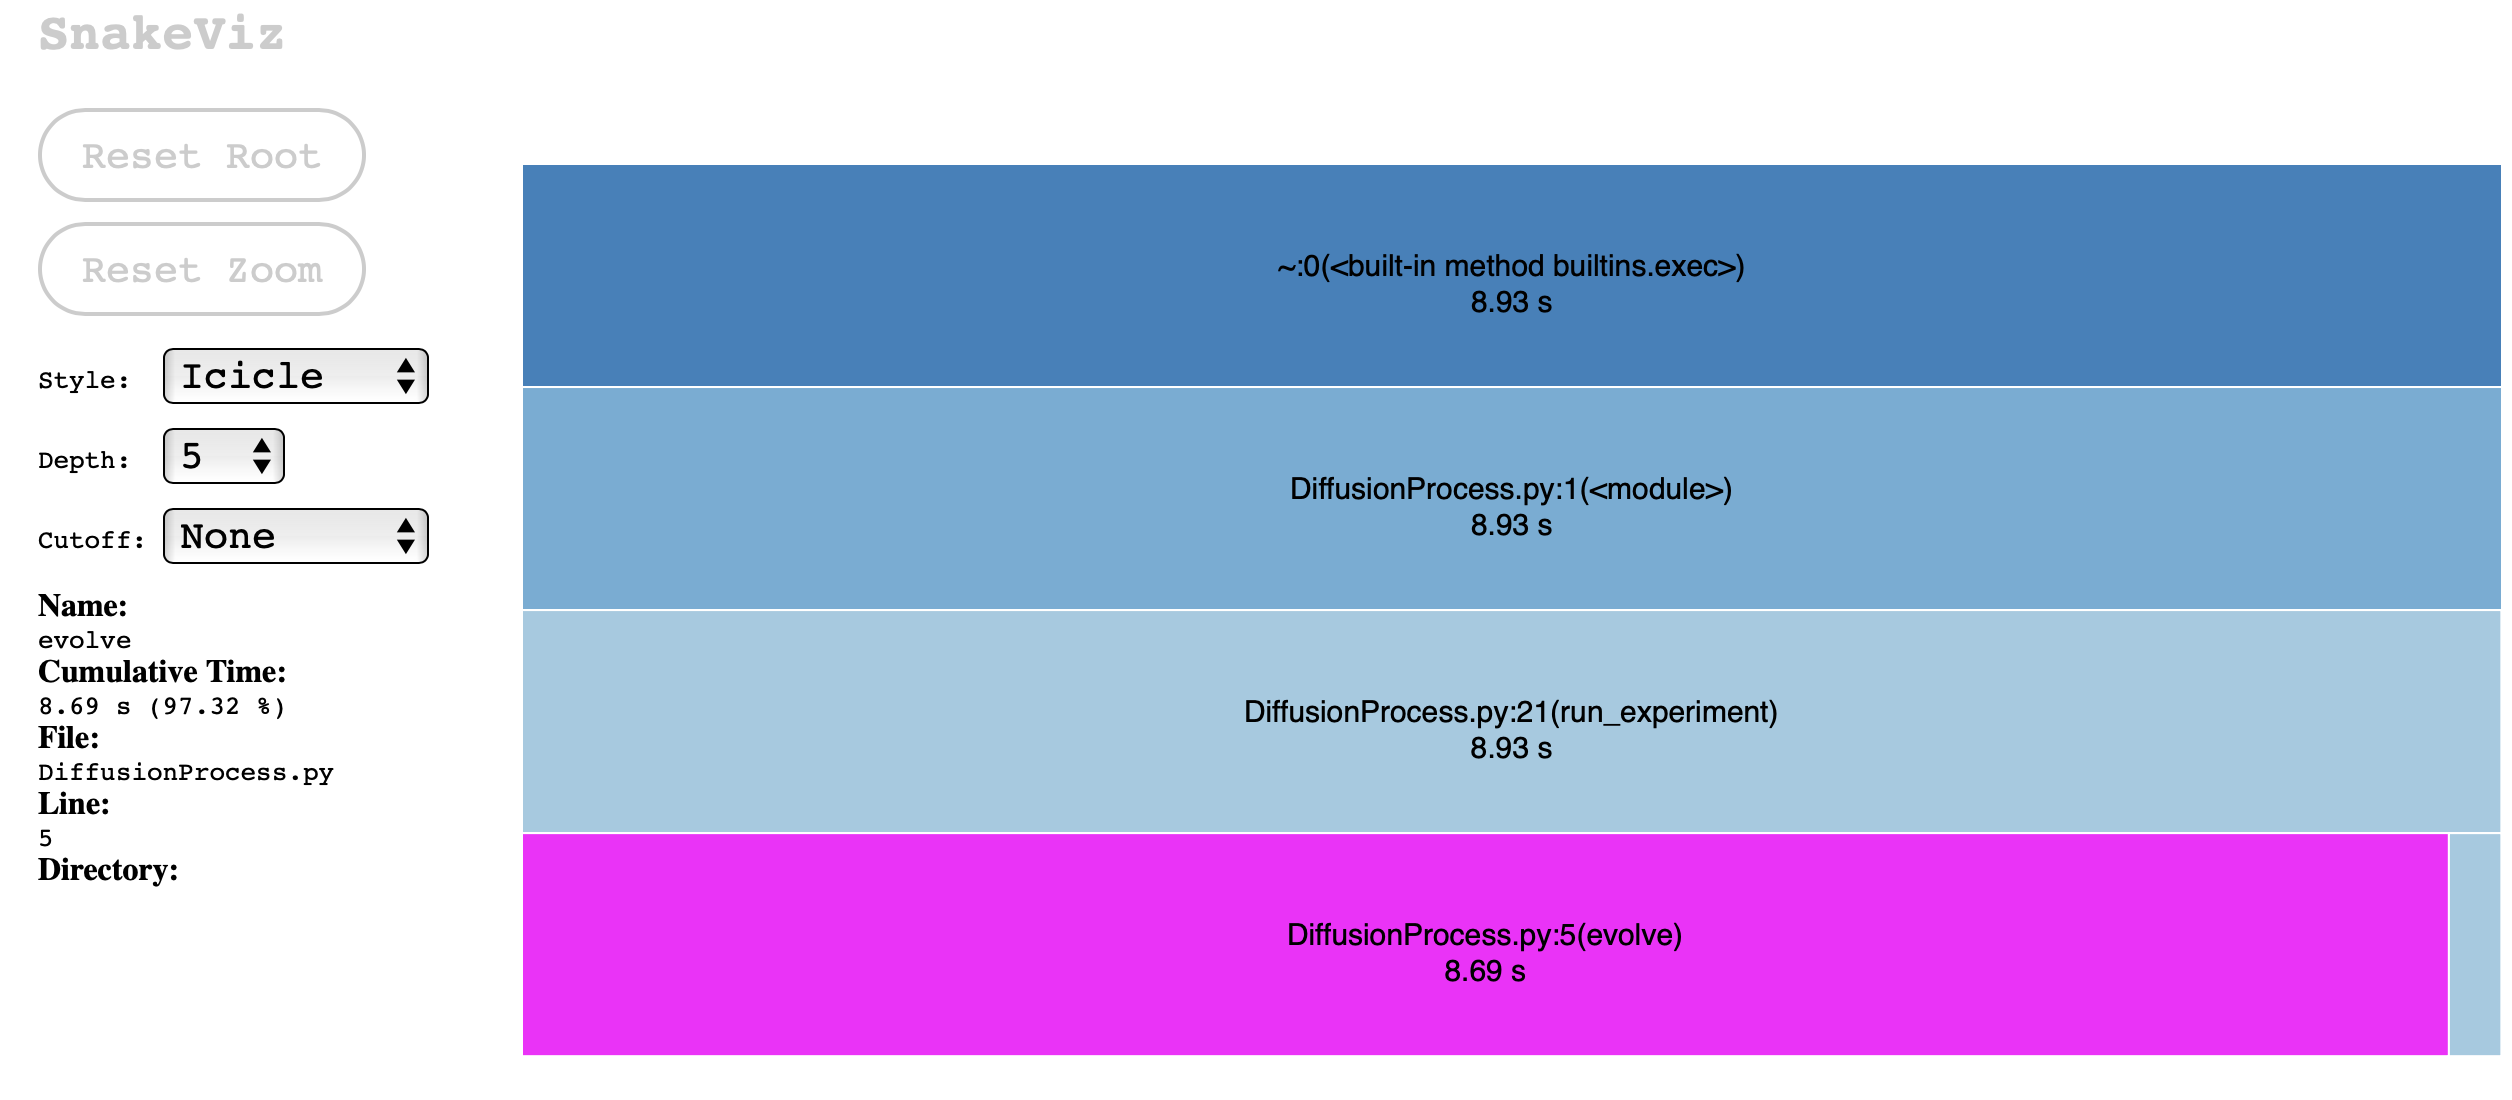
\includegraphics[width=\textwidth]{images/diffusion_snakeviz_view}
  \caption{Diffusion processing snakeviz view}
  \label{fig:diffusion-snakeviz}
\end{figure}

When diving deeper into the \verb|evolve| method using the \verb|line_profiler|, we see the following:

\begin{lstlisting}[language=bash,basicstyle=\tiny\ttfamily]
Timer unit: 1e-06 s

Total time: 29.5351 s
File: DiffusionProcess.py
Function: evolve at line 4

Line #      Hits         Time  Per Hit   % Time  Line Contents
==============================================================
     4                                           @profile
     5                                           def evolve(grid, dt, D=1.0):
     6       100         83.0      0.8      0.0      xmax, ymax = grid_shape
     7     64100      33649.0      0.5      0.1      new_grid = [[0.0] * ymax for x in range(xmax)]
     8     64100       7771.0      0.1      0.0      for i in range(xmax):
     9  41024000    4381699.0      0.1     14.8          for j in range(ymax):
    10  40960000    3618998.0      0.1     12.3              grid_xx = (
    11  40960000    6772659.0      0.2     22.9                  grid[(i + 1) % xmax][j] + grid[(i - 1) % xmax][j] - 2.0 * grid[i][j]
    12                                                       )
    13  40960000    3692418.0      0.1     12.5              grid_yy = (
    14  40960000    6465938.0      0.2     21.9                  grid[i][(j + 1) % ymax] + grid[i][(j - 1) % ymax] - 2.0 * grid[i][j]
    15                                                       )
    16  40960000    4561813.0      0.1     15.4              new_grid[i][j] = grid[i][j] + D * (grid_xx + grid_yy) * dt
    17       100        111.0      1.1      0.0      return new_grid

 29.54 seconds - DiffusionProcess.py:4 - evolve
\end{lstlisting}

Non surprisingly, calculating the grid values takes the most amount of time.
However, around 25\% of the total time spent was used to store the grid values, which seems high.

\subsection{Memory-profile the diffusion code. Use the memory\_profiler and mprof to profile the computation}

\verb|memory_profiler| (one iteration):
\begin{lstlisting}[language=bash,basicstyle=\tiny\ttfamily]
Filename: DiffusionProcess.py

Line #    Mem usage    Increment  Occurrences   Line Contents
=============================================================
     4   25.219 MiB   25.219 MiB           1   @profile
     5                                         def evolve(grid, dt, D=1.0):
     6   25.219 MiB    0.000 MiB           1       xmax, ymax = grid_shape
     7   28.391 MiB    3.172 MiB         641       new_grid = [[0.0] * ymax for x in range(xmax)]
     8   41.016 MiB    0.000 MiB         641       for i in range(xmax):
     9   41.016 MiB    0.094 MiB      410240           for j in range(ymax):
    10   41.016 MiB   12.469 MiB      409600               grid_xx = (
    11   41.016 MiB    0.016 MiB      409600                   grid[(i + 1) % xmax][j] + grid[(i - 1) % xmax][j] - 2.0 * grid[i][j]
    12                                                     )
    13   41.016 MiB    0.016 MiB      409600               grid_yy = (
    14   41.016 MiB    0.016 MiB      409600                   grid[i][(j + 1) % ymax] + grid[i][(j - 1) % ymax] - 2.0 * grid[i][j]
    15                                                     )
    16   41.016 MiB    0.016 MiB      409600               new_grid[i][j] = grid[i][j] + D * (grid_xx + grid_yy) * dt
    17   41.016 MiB    0.000 MiB           1       return new_grid
\end{lstlisting}\vspace{1em}
\verb|mprof| (10 iterations):
\begin{figure}[h!]
  \centering
  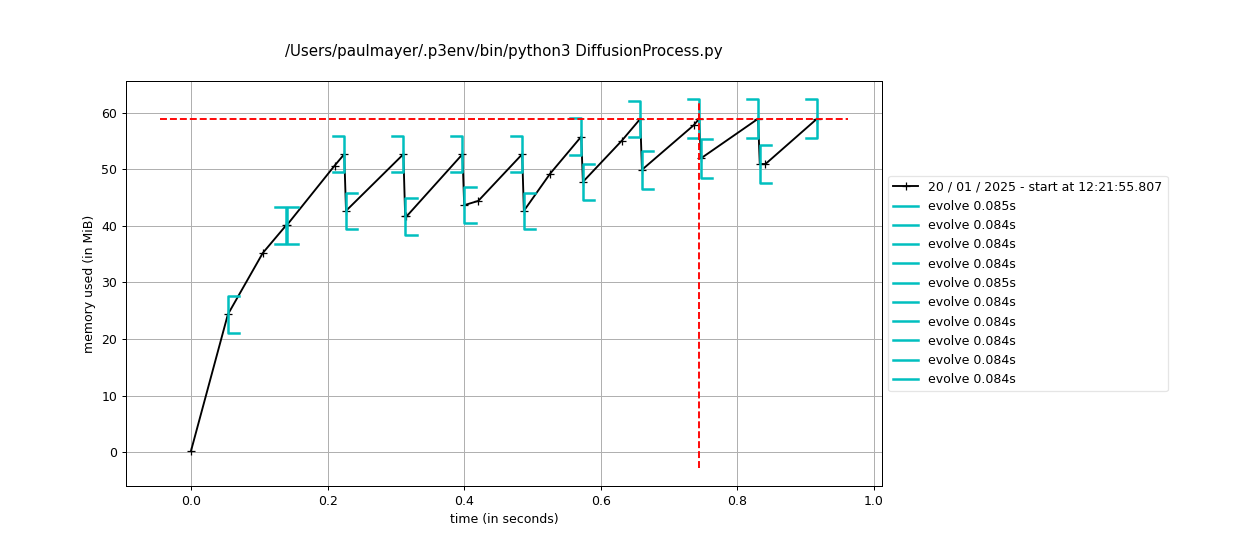
\includegraphics[width=\textwidth]{images/diffusion_mprofile}
  \caption{Diffusion mprof plot}
  \label{fig:diffusion-mprof}
\end{figure}

\newpage
\section{Develop your profiler tool for monitoring CPU percentage use with psutil}
\todo[inline]{3.1: everything}

% content end
%###############################################################################

% TODO: bibliograpghy when needed
% \printbibliography

\end{document}
